% =====================================================================
% AI Academy -- National AI Center
% Software Engineering Final Project -- Team Presentation Deck
%
% HOW TO USE
% ----------
%   1. Edit the CONFIGURATION block (team name, topic, members).
%   2. Replace every \TODO{...} with your content. TODOs render in red,
%      so anything you forgot is visually obvious.
%   3. ~10 slides for a 10-minute talk. Roughly 1 min per slide; the
%      benchmark and architecture slides may take 2 min each.
%   4. Compile with pdfLaTeX (Overleaf works out of the box).
% =====================================================================

\PassOptionsToPackage{dvipsnames}{xcolor}
\documentclass[aspectratio=169,11pt]{beamer}

% ===== CONFIGURATION (edit these) ====================================
\newcommand{\teamname}{AI Food Analyzer Team}
\newcommand{\topicchoice}{Topic 2 -- AI Food Analyzer}
\newcommand{\memberone}{Farhad Budagov}
\newcommand{\membertwo}{Mikayil Hasanov}
\newcommand{\memberthree}{Nihad Gojayev}
\newcommand{\repolink}{github.com/budagovfn/ai-food-analyzer}

\newcommand{\coursecode}{AI-ENG-110}
\newcommand{\coursename}{Software Engineering}
\newcommand{\institution}{AI Academy, National AI Center}
\newcommand{\semester}{Spring 2026}

% ===== PACKAGES ======================================================
\usepackage[T1]{fontenc}
\usepackage[utf8]{inputenc}
\usepackage{xcolor}
\usepackage{tabularx}
\usepackage{booktabs}
\usepackage{listings}
\usepackage{tikz}
\usetikzlibrary{shapes.geometric,arrows.meta,positioning,fit,backgrounds,calc}

% ===== EARLY MACROS ==================================================
\definecolor{accent2}{HTML}{8B0000}
\newcommand{\TODO}[1]{\textcolor{accent2}{\textbf{[TODO: #1]}}}

% ===== BEAMER THEME (custom, no flashy decorations) =================
\usetheme{default}
\usefonttheme{professionalfonts}
\setbeamertemplate{navigation symbols}{}

\definecolor{accent}{HTML}{0B3D91}
\definecolor{soft}{HTML}{F2F4F8}
\definecolor{ok}{HTML}{166534}

\setbeamercolor{title}{fg=accent}
\setbeamercolor{frametitle}{fg=accent}
\setbeamercolor{section in head/foot}{bg=accent,fg=white}
\setbeamercolor{itemize item}{fg=accent}
\setbeamercolor{itemize subitem}{fg=accent}
\setbeamercolor{enumerate item}{fg=accent}
\setbeamercolor{block title}{bg=accent,fg=white}
\setbeamercolor{block body}{bg=soft,fg=black}

\setbeamerfont{title}{size=\Large,series=\bfseries}
\setbeamerfont{frametitle}{size=\large,series=\bfseries}
\setbeamerfont{footline}{size=\tiny}

% Footer with team + slide number
\setbeamertemplate{footline}{%
  \leavevmode%
  \hbox to\paperwidth{\hspace*{2ex}\tiny\textit{\teamname}\hfill%
  \tiny\textit{\coursecode{} -- \semester}\hfill%
  \tiny\insertframenumber/\inserttotalframenumber\hspace*{2ex}}%
  \vskip1pt%
}

% ===== CODE LISTINGS =================================================
\definecolor{codegreen}{rgb}{0,0.55,0}
\definecolor{codepurple}{rgb}{0.55,0,0.78}
\lstdefinestyle{python}{
  language=Python,
  backgroundcolor=\color{soft},
  commentstyle=\color{codegreen},
  keywordstyle=\color{accent},
  stringstyle=\color{codepurple},
  basicstyle=\ttfamily\scriptsize,
  breaklines=true,
  frame=single,
  framerule=0.4pt,
  rulecolor=\color{black!30},
}

% =====================================================================
\begin{document}

% ========== SLIDE 1: TITLE ===========================================
{%
\setbeamertemplate{footline}{}
\begin{frame}[plain]
  \begin{center}
    \vspace{0.6cm}
    {\small \textsc{\institution}}\\[0.2em]
    {\small \textsc{\coursecode{} -- \coursename{} -- \semester{}}}\\[1.2em]
    \rule{0.7\textwidth}{0.6pt}\\[0.4em]
    {\Huge\bfseries\color{accent} \topicchoice}\\[0.4em]
    \rule{0.7\textwidth}{0.6pt}\\[1.2em]
    {\large \teamname}\\[0.6em]
    {\normalsize \memberone\quad\textbullet\quad\membertwo\quad\textbullet\quad\memberthree}\\[1cm]
    {\footnotesize\itshape Final Project Defense -- \TODO{Date}}\\[0.4em]
    {\footnotesize\texttt{\repolink}}
  \end{center}
\end{frame}
}

% ========== SLIDE 2: PROBLEM =========================================
\begin{frame}{The problem in one sentence}
  \begin{block}{What the system does}
    A user uploads a meal photo; we identify the ingredients, look up nutrition facts for each, and return total calories, protein, carbs, and fat, saved to a persistent history.
  \end{block}

  \vspace{0.3em}
  \begin{columns}[T,onlytextwidth]
  \column{0.48\textwidth}
  \textbf{Inputs}
  \begin{itemize}
    \item Meal photo (JPEG/PNG, $\le$5\,MB)
    \item Nothing else -- no manual portion entry
  \end{itemize}

  \column{0.48\textwidth}
  \textbf{Outputs}
  \begin{itemize}
    \item Per-ingredient kcal/protein/carbs/fat + totals (JSON or table)
    \item History record in PostgreSQL
  \end{itemize}
  \end{columns}

  \vspace{0.4em}
  \textbf{Entry points:} \texttt{python -m foodanalyzer analyze <path>} (CLI) \quad+\quad \texttt{POST /analyze}, \texttt{GET /health} (FastAPI)
\end{frame}

% ========== SLIDE 3: ARCHITECTURE ====================================
\begin{frame}{Architecture}
  \textbf{Module map.} The boundary between the \emph{provided} \texttt{ai/} package and \emph{our} SE layer is shown explicitly.

  \vspace{0.2em}
  \begin{center}
  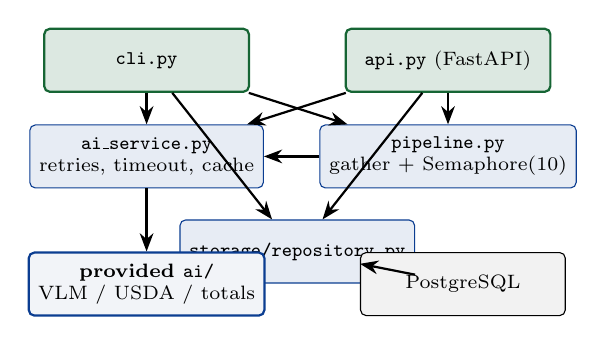
\begin{tikzpicture}[
    node distance=4mm,
    box/.style={draw,rounded corners=2pt,minimum width=2.6cm,minimum height=0.8cm,align=center,font=\scriptsize},
    aibox/.style={box,fill=soft,draw=accent,thick},
    sebox/.style={box,fill=accent!10,draw=accent},
    entry/.style={box,fill=ok!15,draw=ok,thick},
    arrow/.style={-Stealth,thick}
  ]
    \node[entry] (cli) {\texttt{cli.py}};
    \node[entry,right=12mm of cli] (api) {\texttt{api.py} (FastAPI)};

    \node[sebox,below=of cli] (svc) {\texttt{ai\_service.py}\\retries, timeout, cache};
    \node[sebox,below=of api] (conc) {\texttt{pipeline.py}\\gather + Semaphore(10)};

    \node[sebox,below=8mm of $(svc)!0.5!(conc)$] (store) {\texttt{storage/repository.py}};

    \node[aibox,below=8mm of svc] (ai) {\textbf{provided \texttt{ai/}}\\VLM / USDA / totals};

    \node[box,fill=gray!10,right=12mm of ai] (pg) {PostgreSQL};

    \draw[arrow] (cli) -- (svc);
    \draw[arrow] (api) -- (svc);
    \draw[arrow] (api) -- (conc);
    \draw[arrow] (cli) -- (conc);
    \draw[arrow] (conc) -- (svc);
    \draw[arrow] (svc) -- (ai);
    \draw[arrow] (cli) -- (store);
    \draw[arrow] (api) -- (store);
    \draw[arrow] (store) -- (pg);
  \end{tikzpicture}
  \end{center}

  {\footnotesize\textit{Every arrow into \texttt{ai/} passes through \texttt{ai\_service.py} -- nothing else imports a provider directly. Swapping Gemini for Anthropic/OpenAI is a \texttt{.env} change, 0 lines of \texttt{src/} code.}}
\end{frame}

% ========== SLIDE 4: KEY DESIGN DECISIONS ============================
\begin{frame}{Three design decisions we can defend}
  \begin{enumerate}\setlength\itemsep{0.6em}
    \item \textbf{\texttt{asyncio.gather} + Semaphore(10), not a bare thread pool}\\
      \texttt{api.py} is already an async FastAPI app; \texttt{asyncio} lets a slow lookup batch yield the event loop to other requests, which a blocking \texttt{ThreadPoolExecutor.map} inside a route handler would not.
    \item \textbf{A permanent upload directory, not \texttt{NamedTemporaryFile(delete=True)}}\\
      Windows refuses to reopen a file whose handle is still held -- caused a \texttt{PermissionError} on every single request (Slide 6). Rejected alternative: catching the error and retrying, which papers over a design bug instead of fixing it.
    \item \textbf{One shared DB connection pool per process, not one per request}\\
      Opening a fresh \texttt{asyncpg} pool on every \texttt{POST /analyze} risked exhausting Postgres's connection limit under load; a FastAPI \texttt{lifespan} handler now opens it once.
  \end{enumerate}

  \vspace{0.4em}
  \begin{block}{Expect to be asked}
    ``Why not a token-bucket rate limiter instead of a semaphore?'' -- we chose the simpler bound because our real workload (single-digit ingredients per meal) never approaches USDA's 1000 req/h ceiling; see the Limitations slide.
  \end{block}
\end{frame}

% ========== SLIDE 5: CONCURRENCY (THE BENCHMARK) =====================
\begin{frame}{Concurrency: the benchmark}
  \textbf{Workload:} 10 distinct ingredients (rice, chicken, broccoli, salmon, potato, egg, salad, pasta, tomato, cheese), fresh \texttt{NutritionService} each run so neither side gets a cache hit.

  \vspace{0.4em}
  \begin{center}\small
  \begin{tabular}{lcc}
    \toprule
    & \textbf{Sequential} & \textbf{Concurrent (sem=10)} \\
    \midrule
    Wall-clock (s) & 15.69 & 3.16 \\
    Speedup        & 1.0$\times$ & \textbf{4.96$\times$} \\
    USDA 429s      & 0  & 0 \\
    \bottomrule
  \end{tabular}
  \end{center}

  \vspace{0.4em}
  \textbf{Bottleneck named:} network round-trip time to USDA per ingredient -- the lookup is I/O-bound, not CPU-bound.\\
  \textbf{What didn't reach $10\times$:} with $N=10$ = semaphore bound, all lookups start together, so wall-clock is set by the \emph{slowest} single response, not an even $1/10$ share -- real latency variance means we land at $\sim$5$\times$, not 10$\times$.\\
  \textbf{Reproduce with:} \texttt{python scripts/benchmark\_concurrency.py} (needs a real \texttt{USDA\_API\_KEY}).

  \vspace{0.3em}
  {\footnotesize\textit{Numbers must reproduce from the README. Have the exact command line ready.}}
\end{frame}

% ========== SLIDE 6: ROBUSTNESS STORY ================================
\begin{frame}{Robustness: two failure modes, one loud and one silent}
  \begin{columns}[T,onlytextwidth]
  \column{0.48\textwidth}
  \textbf{Loud: 500 on every request}
  \begin{itemize}\setlength\itemsep{0.2em}\small
    \item \texttt{NamedTemporaryFile(delete=True)} holds its handle; \texttt{ai/} reopens the image by path; Windows refuses the second handle.
    \item The traceback named it exactly: \texttt{PermissionError: [WinError 32]}.
    \item Fix: a permanent UUID-named path under \texttt{data/uploads/}, unlinked on success \emph{and} failure.
  \end{itemize}

  \column{0.48\textwidth}
  \textbf{Silent: 200 OK, wrong number}
  \begin{itemize}\setlength\itemsep{0.2em}\small
    \item \texttt{/analyze} reported \textbf{1975\,kcal} for a 240\,g plate --- valid schema, correct types, nothing failed.
    \item Atwater on that same response gives \textbf{459}\,kcal. Ratio \textbf{4.30}; kJ per kcal is \textbf{4.184}.
    \item \texttt{ai/nutrition.py} drops \texttt{unitName}; USDA sends \texttt{Energy} twice and KJ wins. Fixed in \emph{our} layer --- \S4.8 forbids editing \texttt{ai/}.
  \end{itemize}
  \end{columns}

  \vspace{0.2em}
  \begin{block}{Why the silent one matters more}
    \small Retries, timeouts and graceful degradation all handle calls that \emph{fail}; none engage when a call succeeds with a plausible-looking number. A physical invariant caught it, not another test.
  \end{block}
\end{frame}

% ========== SLIDE 7: DEMO ============================================
\begin{frame}[fragile]{Live demo --- from a clean clone}
  \begin{block}{What we will run}
    The whole system brought up from the repository with a single command, then the same photo through both front doors, showing identical totals.
  \end{block}

  \vspace{0.3em}
  \begin{lstlisting}[style=python,language=bash,numbers=none]
$ docker compose up --build     # API + PostgreSQL 16, one command

$ curl.exe http://localhost:8000/health
$ curl.exe -F "file=@data/rice_chicken_broccoli.png" http://localhost:8000/analyze

$ docker compose run --rm api python -m foodanalyzer analyze data/rice_chicken_broccoli.png
  \end{lstlisting}

  \vspace{0.2em}
  \begin{itemize}\setlength\itemsep{0.2em}\small
    \item Same ingredients, same totals, two front doors --- both entry points share one business-logic path.
    \item The image carries the CLI and the offline demo as well as the server: \texttt{docker compose run -{}-rm api python demo\_ai.py -{}-offline}.
    \item \texttt{data/no\_meal\_blue.png} shows the graceful \texttt{meal\_recognized=false} branch, not a crash.
  \end{itemize}
\end{frame}

% ========== SLIDE 8: TESTING =========================================
\begin{frame}{Testing}
  \begin{columns}[T,onlytextwidth]
  \column{0.55\textwidth}
  \textbf{Coverage \& shape}
  \begin{itemize}\setlength\itemsep{0.3em}
    \item \textbf{93\,\%} on \texttt{src/}, \textbf{64\,\%} with \texttt{ai/}; \textbf{102} tests, offline
    \item \texttt{api.py} 90\,\%, \texttt{cli.py} 84\,\%, \texttt{ai\_service.py} 97\,\%; the rest of \texttt{src/} 100\,\%
    \item Uncovered remainder: the provided \texttt{ai/providers/} adapters
    \item Provided \texttt{test\_ai\_smoke.py} untouched, 29 passing
  \end{itemize}

  \column{0.42\textwidth}
  \textbf{Four tests worth calling out}
  \begin{itemize}\setlength\itemsep{0.25em}\small
    \item Happy path: all ingredients priced
    \item Concurrency: one lookup fails, batch survives
    \item Retry-exhausted $\to$ \texttt{AIServiceError}, never a raw timeout
    \item Unit audit: the 1975\,kcal payload, wrong before the fix, consistent after
  \end{itemize}
  \end{columns}

  \vspace{0.3em}
  \begin{block}{Honesty note}
    \small Our timing test used to be vacuous --- an autouse fixture disabled \texttt{time.sleep} globally, killing the delay it measures. Now fixed, and verified by sabotage: sequential code fails in 2.5\,s where it used to pass in 0.07\,s.
  \end{block}
\end{frame}

% ========== SLIDE 9: LIMITATIONS + FUTURE ============================
\begin{frame}{Limitations \& what we'd do next}
  \textbf{Where the system is brittle today}
  \begin{itemize}\setlength\itemsep{0.3em}
    \item \textbf{Identification is the weakest link.} On \texttt{rice\_chicken.png} the VLM reported a ``grilled beef patty'', and portions come back as round numbers. Our unit audit catches a wrong \emph{unit}, never a wrong \emph{ingredient}.
    \item No load test against concurrent \emph{requests} (only concurrent lookups within one request); the likeliest failure on a busy day is Postgres pool exhaustion at \texttt{max\_size=5}, not the AI layer.
    \item Single-provider, no failover --- a Gemini outage or an invalid USDA key fails that stage after 3 retries, with no fallback provider.
  \end{itemize}

  \vspace{0.4em}
  \textbf{Given another week we would}
  \begin{enumerate}\setlength\itemsep{0.3em}
    \item Write a contract test for the USDA adapter: one recorded payload, replayed offline. It would have caught the kilojoule defect on day one.
    \item Run a real load test against the Docker image, then add a second VLM/nutrition provider for failover.
  \end{enumerate}
\end{frame}

% ========== SLIDE 10: TEAM CONTRIBUTIONS =============================
\begin{frame}{Team contributions}
  \begin{center}\footnotesize
  \begin{tabularx}{\linewidth}{lXl}
    \toprule
    \textbf{Member} & \textbf{Primary ownership} & \textbf{Commits} \\
    \midrule
    \memberone   & Config and storage layers, HTTP API fixes, Docker hardening, unit-audit provider, git/PR workflow, report \& slides & 33/47 \textit{(17/29)} \\
    \membertwo   & AI-service wrapper (retry/timeout/cache), concurrency pipeline, FastAPI endpoint, Dockerfile \& compose & 9/47 \textit{(9/29)} \\
    \memberthree & API and CLI test suites, \texttt{README}, pull-request review and merges & 5/47 \textit{(3/29)} \\
    \bottomrule
  \end{tabularx}\\[0.3em]
  {\scriptsize From \texttt{git shortlog -sn} with the repository's \texttt{.mailmap}, which collapses the several git identities we each committed under. In italics: excluding merge commits --- 16 of the 18 merges on \texttt{main} are Farhad's, from running the PR workflow, and count towards a total without being authored code.}
  \end{center}

  \vspace{0.2em}
  {\small\textbf{AI tool use:} Claude reviewed and hardened the Docker PR, fixed two failing tests, found the kilojoule defect on Slide 6 and wrote the provider guarding against it, and drafted this deck and the report from our commit history. Every approval and merge was made by a team member; full disclosure in \S9 of the report.}

  \vspace{0.2em}
  \begin{block}{We can all answer:}
    \small Pick any file in the repo --- whoever owns it will walk you through it.
  \end{block}
\end{frame}

% ========== SLIDE 11: THANK YOU / Q&A ================================
{%
\setbeamertemplate{footline}{}
\begin{frame}[plain]
  \begin{center}
    \vspace{1cm}
    {\Huge\bfseries\color{accent} Questions?}\\[1.2em]
    \rule{0.5\textwidth}{0.6pt}\\[1.2em]
    {\large \teamname}\\[0.6em]
    {\normalsize \texttt{\repolink}}\\[1cm]
    {\footnotesize\itshape ``We can walk through any file in the repo.''}
  \end{center}
\end{frame}
}

\end{document}
